% Main document for the report (XeLaTeX recommended on Overleaf)
\documentclass[12pt,a4paper]{report}

% XeLaTeX: Unicode + Vietnamese
\usepackage{fontspec}
\usepackage{polyglossia}
\setdefaultlanguage{vietnamese}
% Fonts (TeX Gyre families are available on TeX Live/Overleaf)
\setmainfont{TeX Gyre Termes}
\setsansfont{TeX Gyre Heros}
\setmonofont{TeX Gyre Cursor}

% Layout and links
\usepackage[top=2.5cm, bottom=2.5cm, left=3.5cm, right=2cm]{geometry}
\usepackage{setspace}\onehalfspacing
\usepackage{hyperref}\hypersetup{colorlinks=true, linkcolor=blue, urlcolor=cyan}

% Shared packages/styles
% Shared packages and styles
\usepackage{graphicx}
\usepackage{xcolor}
\usepackage{tikz}
\usetikzlibrary{shapes.geometric, arrows.meta, positioning, calc, shadows}
\usepackage{tabularx}
\usepackage{booktabs}
\usepackage{listings}
\usepackage{float}
\usepackage{subcaption}
\usepackage{enumitem}
\setlist{nosep}
\usepackage{amsmath, amssymb}
\usepackage{algorithm}
\usepackage{algpseudocode}

% Listings
\lstset{basicstyle=\ttfamily\footnotesize, breaklines=true, frame=single, numbers=left, numberstyle=\tiny, tabsize=2, showstringspaces=false}

% TikZ styles and helpers
\tikzset{block/.style={rectangle,draw,fill=blue!8,text width=8em,align=center,rounded corners,minimum height=3.2em,drop shadow},
         smallblock/.style={rectangle,draw,fill=blue!8,align=center,rounded corners,minimum height=2.2em,inner sep=4pt},
         entity/.style={rectangle,draw,fill=cyan!6,rounded corners,align=left,minimum width=14em},
         actor/.style={draw,thick},
         boundary/.style={draw,rounded corners,thick,dashed,gray!70,inner sep=8pt},
         note/.style={draw,fill=red!5,rounded corners,align=left},
         part/.style={rectangle,draw,rounded corners,fill=gray!8,minimum height=1.2em,align=center,inner sep=6pt},
         lifeline/.style={densely dashed,gray!70},
         exec/.style={rectangle,draw,fill=gray!15,minimum width=2.2em,minimum height=0.6cm},
         arrow/.style={-{Stealth[length=2.6mm]},thick}}
\newcommand{\placeholder}[2]{\begin{tikzpicture}\fill[white](0,0)rectangle(#1,#2);\draw[gray!50](0,0)rectangle(#1,#2);\node[gray]at(#1/2,#2/2){Placeholder Image};\end{tikzpicture}}

% Default image path
\graphicspath{{img/}}


% Metadata (Sửa tương ứng trước khi in)
\newcommand{\TenTruong}{TRƯỜNG ………}
\newcommand{\TenKhoa}{KHOA/VIỆN ………}
\newcommand{\TenMon}{BÁO CÁO ĐỒ ÁN MÔN HỌC}
\newcommand{\TenDeTai}{HỆ THỐNG CHIA SẺ FILE VỚI MÃ HÓA CLIENT-SIDE SỬ DỤNG BLOCKCHAIN}
\newcommand{\GVHD}{TS. ……………}
\newcommand{\SinhVien}{………………}
\newcommand{\MSSV}{……….}
\newcommand{\Lop}{……….}
\newcommand{\DiaDiem}{Hà Nội}
\newcommand{\Nam}{2025}

\begin{document}

\begin{titlepage}
  \centering
  \vspace*{-1cm}
  
  {\large\bfseries \TenTruong\\}
  \vspace{0.2cm}
  {\large\bfseries \TenKhoa\\}
  
  \vspace{0.8cm}
  
  % Logo
  \IfFileExists{img/logo.jpg}%
    {
\includegraphics[width=3.5cm]{img/logo.jpg}}%
    {}
  
  \vspace{0.8cm}
  
  {\large\bfseries \TenMon\\}
  \vspace{0.3cm}
  {\normalsize\bfseries \HocPhan\\}
  \vspace{0.3cm}
  {\normalsize \LopNhom\\}
  
  \vspace{0.8cm}
  
  {\Large\bfseries \TenDeTai\\}
  
  \vspace{1.2cm}
  
  % Thành viên nhóm table
  {\small
  \textbf{Thành viên nhóm}
  
  \vspace{0.3cm}
  
  \begin{tabular}{|c|c|c|}
    \hline
    \textbf{MSSV} & \textbf{Họ và tên} & \textbf{Nhiệm vụ} \\
    \hline
    23010864 & Hoàng Tiến Đạt & 11 \\
    \hline
    23010876 & Tô Thị Thùy Dương & 11 \\
    \hline
     &  &  \\
    \hline
  \end{tabular}
  }
  
  \vspace{1cm}
  
  {\normalsize \textbf{GVHD: \GVHD}}
  
  \vfill
  
  {\normalsize \textbf{\DiaDiem, tháng 10 năm \Nam}}

\end{titlepage}


\chapter*{Lời cảm ơn}
\addcontentsline{toc}{chapter}{Lời cảm ơn}
Tác giả xin chân thành cảm ơn giảng viên hướng dẫn, các thầy cô bộ môn và bạn bè đã hỗ trợ trong suốt quá trình thực hiện đề tài. Xin gửi lời cảm ơn tới cộng đồng mã nguồn mở đã cung cấp các thư viện và tài liệu tham khảo giúp dự án hoàn thiện.

\vspace{0.6cm}
\hfill \textit{\DiaDiem, ngày … tháng … năm \Nam}\par
\hfill \textit{Sinh viên thực hiện}

\chapter*{Lời cam đoan}
\addcontentsline{toc}{chapter}{Lời cam đoan}
Tôi xin cam đoan báo cáo này là kết quả nghiên cứu và triển khai của bản thân trong phạm vi môn học. Các nội dung trích dẫn đều được ghi rõ nguồn. Nếu có sai phạm, tôi xin hoàn toàn chịu trách nhiệm.

\chapter*{Tóm tắt}
\addcontentsline{toc}{chapter}{Tóm tắt}
Đề tài xây dựng hệ thống chia sẻ tệp tin bảo mật theo mô hình zero‑knowledge: dữ liệu được \textbf{mã hóa phía client} bằng AES‑256‑GCM, máy chủ chỉ lưu ciphertext và metadata. Quyền truy cập được cấp qua \textbf{mã chia sẻ (token)} có thời hạn. Người dùng đăng nhập bằng \textbf{chữ ký ví Ethereum (MetaMask)} để xác thực mà không cần mật khẩu. Báo cáo trình bày lý do lựa chọn thuật toán, thiết kế hệ thống, phân tích bảo mật, luồng thuật toán chi tiết, hiện thực hoá và đánh giá.


\tableofcontents
\listoffigures
\listoftables
\chapter*{Danh mục từ viết tắt}
\addcontentsline{toc}{chapter}{Danh mục từ viết tắt}
\begin{tabular}{@{}ll}
\textbf{AES} & Advanced Encryption Standard \\
\textbf{GCM} & Galois/Counter Mode \\
\textbf{PBKDF2} & Password‑Based Key Derivation Function 2 \\
\textbf{JWT} & JSON Web Token \\
\textbf{CID} & Content Identifier \\
\textbf{API} & Application Programming Interface \\
\textbf{CSRF} & Cross‑Site Request Forgery \\
\textbf{KDF} & Key Derivation Function \\
\textbf{UI} & User Interface \\
\end{tabular}


\chapter{Tổng quan đề tài}

\section{Bối cảnh và động lực}
Trong kỷ nguyên dữ liệu, nhu cầu \textit{chia sẻ an toàn} và \textit{kiểm soát quyền riêng tư} ngày càng cấp thiết. Mô hình lưu trữ tập trung có nguy cơ lộ lọt dữ liệu và phụ thuộc nhà cung cấp. Tiếp cận \textbf{client‑side encryption} đảm bảo khoá bí mật không rời thiết bị người dùng, giảm thiểu rủi ro xâm phạm phía máy chủ.

\section{Mục tiêu}
\begin{itemize}
  \item Xây dựng hệ thống chia sẻ tệp với \textbf{mã hóa client‑side AES‑256‑GCM}.
  \item Cấp quyền truy cập qua \textbf{token} có TTL, có thể thu hồi.
  \item Xác thực đăng nhập bằng \textbf{chữ ký ví Ethereum (MetaMask)}.
  \item Lưu ciphertext và metadata an toàn; máy chủ \textbf{không biết khoá giải mã}.
\end{itemize}

\section{Phạm vi}
\subsection*{Trong phạm vi}
Web app Next.js, mã hóa bằng Web Crypto API, lưu ciphertext local (demo), metadata trong SQLite, quản lý token và phiên đăng nhập bằng JWT cookie.

\subsection*{Ngoài phạm vi}
Triển khai IPFS/Filecoin thực tế, hợp đồng thông minh on‑chain và ứng dụng di động nằm ngoài phạm vi môn học (để mở hướng phát triển).


\chapter{Cơ sở lý thuyết}

\section{Lý do chọn AES‑256‑GCM}
\textbf{AES} là chuẩn mực công nghiệp, được tăng tốc phần cứng và hỗ trợ native bởi Web Crypto API. \textbf{GCM} cung cấp cả bảo mật \textit{bí mật} lẫn \textit{toàn vẹn/xác thực} (AEAD). Kích thước IV 96‑bit tiêu chuẩn giúp hiệu năng tốt và đơn giản khi triển khai. Với khoá 256‑bit, không có tấn công thực tế tốt hơn vét cạn.

\section{Tổng quan AES}
AES là mã khối kích thước 128‑bit, cấu trúc SPN với các bước \textit{SubBytes}, \textit{ShiftRows}, \textit{MixColumns}, \textit{AddRoundKey}. Số vòng phụ thuộc độ dài khoá (14 vòng cho 256‑bit).

\begin{figure}[H]
  \centering
  \begin{tikzpicture}[node distance=1.2cm]
    \node (pt) [block] {Plaintext 128‑bit};
    \node (rk0) [smallblock, below=of pt] {AddRoundKey};
    \node (round) [smallblock, below=of rk0] {SubBytes → ShiftRows → MixColumns → AddRoundKey};
    \node (dots) [below=0.2cm of round] {$\times$ (Nr−1) vòng};
    \node (final) [smallblock, below=0.2cm of dots] {SubBytes → ShiftRows → AddRoundKey};
    \node (ct) [block, below=of final] {Ciphertext 128‑bit};
    \draw[arrow] (pt) -- (rk0);
    \draw[arrow] (rk0) -- (round);
    \draw[arrow] (round) -- (dots);
    \draw[arrow] (dots) -- (final);
    \draw[arrow] (final) -- (ct);
  \end{tikzpicture}
  \caption{Cấu trúc vòng AES (minh hoạ)}
\end{figure}

\section{GCM và tính xác thực}
GCM kết hợp CTR để mã hóa và GHASH để tính nhãn xác thực (tag). Đầu vào gồm khoá bí mật, IV (không lặp), dữ liệu kèm theo AAD (tuỳ chọn), bản rõ; đầu ra gồm bản mã và tag xác thực. Sai IV hoặc thay đổi dữ liệu khiến giải mã thất bại.

\section{PBKDF2 và bao bọc khoá}
Khi người dùng chọn passphrase, hệ thống dùng PBKDF2‑HMAC‑SHA‑256 (200k vòng) sinh khoá dẫn xuất để \textbf{bao bọc khoá AES} bằng AES‑GCM (key wrapping). Lưu trữ: salt (16B), ivWrap (12B) và wrappedKey. Nếu ở chế độ demo, có thể lưu khoá dạng base64 (không khuyến nghị sản xuất).


\chapter{Phân tích và thiết kế hệ thống}

\section{Kiến trúc tổng thể}
\begin{figure}[H]
  \centering
  \begin{tikzpicture}[node distance=1.6cm]
    \node (client) [block, text width=12em] {Client (Browser)\\Web Crypto AES‑GCM\\MetaMask};
    \node (api) [block, right=5.0cm of client, text width=13em] {Backend (Next.js)\\JWT session, CSRF\\SQLite metadata};
    \node (store) [block, below=2.0cm of api, text width=13em] {Storage (Local/Stub IPFS)\\Ciphertext by CID};
    % Two arcs between the same nodes to avoid label overlapping
    \draw[arrow] (client.east) to[out=5,in=175,looseness=0.95] node[above,pos=0.55,yshift=6]{Đăng nhập: ký nonce} (api.west);
    \draw[arrow] (client.east) to[out=-10,in=185,looseness=1.15] node[below,pos=0.55,yshift=-6]{Upload ciphertext} (api.west);
    % Vertical API <-> Storage
    \draw[arrow] (api.south) -- node[right,xshift=6]{PUT/GET by CID} (store.north);
    % Client -> Storage with a bend
    \draw[arrow] (client.south east) to[out=-30,in=180] node[below,pos=0.6,yshift=-6]{Tải xuống + giải mã} (store.west);
  \end{tikzpicture}
  \caption{Kiến trúc hệ thống và luồng chính}
\end{figure}

\section{Thiết kế bảo mật}
\begin{itemize}
  \item \textbf{Zero‑knowledge server}: máy chủ không giữ khoá giải mã.
  \item \textbf{AEAD}: AES‑GCM bảo vệ bí mật và toàn vẹn dữ liệu.
  \item \textbf{IV 96‑bit ngẫu nhiên}: sinh mới mỗi lần mã hoá.
  \item \textbf{Token TTL + thu hồi}: giảm cửa sổ tấn công.
  \item \textbf{CSRF + SameSite Cookie}: bảo vệ yêu cầu thay đổi trạng thái.
  \item \textbf{Đăng nhập bằng chữ ký}: loại bỏ mật khẩu phía server.
\end{itemize}

\section{Sơ đồ luồng Upload}
\begin{figure}[H]
  \centering
  \begin{tikzpicture}[node distance=1.1cm]
    \node (s0) [smallblock, text width=16em] {Chọn tệp, nhập tiêu đề và (tuỳ chọn) passphrase};
    \node (s1) [smallblock, below=of s0] {Sinh IV 12B, sinh khoá AES‑GCM 256‑bit};
    \node (s2) [smallblock, below=of s1] {Mã hoá bản rõ → ciphertext};
    \node (s3) [smallblock, below=of s2, text width=16em] {Nếu có passphrase: PBKDF2(200k) → wrap khoá bằng AES‑GCM};
    \node (s4) [smallblock, below=of s3] {Upload ciphertext → nhận CID};
    \node (s5) [smallblock, below=of s4, text width=16em] {Ghi metadata (IV, CID, mô tả, và wrappedKey hoặc rawKeyBase64)};
    \node (s6) [smallblock, below=of s5] {Phát hành token (UUID, TTL)};
    \foreach \i/\j in {s0/s1,s1/s2,s2/s3,s3/s4,s4/s5,s5/s6} {\draw[arrow] (\i) -- (\j);}
  \end{tikzpicture}
  \caption{Luồng tải lên và phát hành token}
\end{figure}

\section{Sơ đồ luồng Download}
\begin{figure}[H]
  \centering
  \begin{tikzpicture}[node distance=1.1cm]
    \node (d0) [smallblock, text width=16em] {Nhập token → server kiểm tra hạn, thu hồi, đối chiếu file};
    \node (d1) [smallblock, below=of d0, text width=16em] {Nhận metadata: IV, CID, wrappedKey hoặc rawKeyBase64};
    \node (d2) [smallblock, below=of d1] {Tải ciphertext theo CID};
    \node (d3) [smallblock, below=of d2, text width=16em] {Nếu wrapped: KDF từ passphrase, giải bao bọc khoá};
    \node (d4) [smallblock, below=of d3] {Giải mã AES‑GCM bằng IV + khoá};
    \node (d5) [smallblock, below=of d4] {Tải file rõ về máy người dùng};
    \foreach \i/\j in {d0/d1,d1/d2,d2/d3,d3/d4,d4/d5} {\draw[arrow] (\i) -- (\j);}
  \end{tikzpicture}
  \caption{Luồng tải xuống và giải mã}
\end{figure}

\section{Sơ đồ Use Case}
\begin{figure}[H]
  \centering
  \begin{tikzpicture}[node distance=1.0cm]
    % System boundary
    \node (boundary) [boundary, minimum width=14cm, minimum height=8cm] {};
    % Actor
    \node[actor, left=2cm of boundary.west] (user) {};
    % Draw stick figure
    \begin{scope}[shift={(user)}]
      \draw (0,0) circle [radius=0.4];
      \draw (0,-0.4) -- (0,-1.6);
      \draw (-0.7,-0.8) -- (0.7,-0.8);
      \draw (-0.6,-2.4) -- (0,-1.6) -- (0.6,-2.4);
    \end{scope}
    \node[left=0.2cm of user] {Người dùng};
    % Use cases inside boundary
    \node (uc1) [draw, ellipse, align=center, minimum width=6.2cm, minimum height=1.2cm] at ($(boundary.center)+(0,2.4)$) {Đăng nhập bằng ví (ký nonce)};
    \node (uc2) [draw, ellipse, align=center, minimum width=6.2cm, minimum height=1.2cm] at ($(boundary.center)+(0,1.0)$) {Upload (Mã hoá + Lưu ciphertext)};
    \node (uc3) [draw, ellipse, align=center, minimum width=6.2cm, minimum height=1.2cm] at ($(boundary.center)+(-3.5,-0.4)$) {Phát hành token};
    \node (uc4) [draw, ellipse, align=center, minimum width=6.2cm, minimum height=1.2cm] at ($(boundary.center)+(3.5,-0.4)$) {Thu hồi token};
    \node (uc5) [draw, ellipse, align=center, minimum width=6.2cm, minimum height=1.2cm] at ($(boundary.center)+(0,-1.8)$) {Download \& Decrypt};
    % Associations
    \draw (user.east) -- (uc1.west);
    \draw (user.east) -- (uc2.west);
    \draw (user.east) -- (uc3.west);
    \draw (user.east) -- (uc4.west);
    \draw (user.east) -- (uc5.west);
  \end{tikzpicture}
  \caption{Sơ đồ ca sử dụng (Use Case)}
\end{figure}

\section{Sơ đồ ERD (rút gọn)}
\begin{figure}[H]
  \centering
  \begin{tikzpicture}[node distance=2.2cm]
    \node (files) [entity] {\textbf{files}\newline id (PK)\newline owner\_address\newline title, description\newline cid, name, mime\newline size\_bytes\newline iv, salt, iv\_wrap, wrapped\_key\newline raw\_key\_base64\newline created\_at};
    \node (tokens) [entity, right=4.8cm of files] {\textbf{tokens}\newline token (PK)\newline file\_id (FK→files.id)\newline issued\_to\_address\newline expires\_at\newline revoked\newline created\_at};
    \draw[arrow] (files) -- node[above]{1 : N} (tokens);
  \end{tikzpicture}
  \caption{Sơ đồ thực thể–quan hệ giữa files và tokens}
\end{figure}

\section{DFD / Threat Model tổng quát}
\begin{figure}[H]
  \centering
  \begin{tikzpicture}[node distance=1.4cm]
    \node (cbound) [boundary, minimum width=4.6cm, minimum height=5.0cm] {};
    \node (client) [block, text width=10.5em] at (cbound.center) {Client\\AES‑GCM, PBKDF2\\MetaMask};
    \node (api) [block, right=5.0cm of client, text width=12em] {API/Backend\\JWT/CSRF\\SQLite};
    \node (store) [block, below=of api, text width=12em] {Storage\\Ciphertext by CID};
    \draw[arrow] (client.east) to[out=5,in=175] node[above,pos=0.55,yshift=6]{Sign nonce} (api.west);
    \draw[arrow] (client.east) to[out=-10,in=185] node[below,pos=0.55,yshift=-6]{Upload ciphertext} (api.west);
    \draw[arrow] (api.south) -- node[right,xshift=6]{PUT/GET CID} (store.north);
    \draw[arrow,gray] (client.south east) to[out=-30,in=180] node[below,pos=0.6,yshift=-6]{Download + Decrypt} (store.west);
    % Threat notes
    \node[note, above=0.1cm of api] (t1) {CSRF on state-changing endpoints};
    \node[note, right=0.3cm of store] (t2) {Token leak / replay};
    \node[note, below=0.1cm of cbound] (t3) {IV reuse risk: 96-bit random IV per file};
  \end{tikzpicture}
  \caption{DFD và ghi chú đe doạ (CSRF, token leak, IV reuse)}
\end{figure}

\section{Bản đồ API}
\begin{figure}[H]
  \centering
  \begin{tikzpicture}[node distance=1.0cm]
    \node (api) [block, text width=12em] {API (Next.js)};
    \node (a1) [smallblock, above left=0.9cm and 2.6cm of api] {POST /api/auth/start};
    \node (a2) [smallblock, above right=0.9cm and 2.6cm of api] {POST /api/auth/verify};
    \node (a3) [smallblock, left=2.8cm of api] {POST /api/storage/upload};
    \node (a4) [smallblock, right=2.8cm of api] {GET /api/storage/get};
    \node (a5) [smallblock, below left=0.9cm and 2.6cm of api] {POST /api/files};
    \node (a6) [smallblock, below=1.0cm of api] {POST /api/tokens/validate};
    \node (a7) [smallblock, below right=0.9cm and 2.6cm of api] {POST /api/tokens/revoke};
    \foreach \x in {a1,a2,a3,a4,a5,a6,a7} {\draw[arrow] (api) -- (\x);}  
  \end{tikzpicture}
  \caption{Các route API chính}
\end{figure}

\section{Sequence: Đăng nhập (ký nonce)}
\begin{figure}[H]
  \centering
  \begin{tikzpicture}[x=1cm,y=1cm]
    % Participants
    \node (user) at (0,0) [part,text width=8em]{Người dùng};
    \node (client) at (6,0) [part,text width=10em]{Trình duyệt / MetaMask};
    \node (server) at (13,0) [part,text width=10.5em]{Backend (Auth API)};
    % Lifelines
    \draw[lifeline] (user.south) -- ++(0,-8.6);
    \draw[lifeline] (client.south) -- ++(0,-8.6);
    \draw[lifeline] (server.south) -- ++(0,-8.6);
    % Messages
    \draw[arrow] ([yshift=-0.8cm]user.south) -- node[above]{Mở ứng dụng} ([yshift=-0.8cm]client.south);
    \draw[arrow] ([yshift=-1.8cm]client.south) -- node[above]{POST /api/auth/start} ([yshift=-1.8cm]server.south);
    \draw[arrow] ([yshift=-2.6cm]server.south) -- node[above]{Set-Cookie: nonce} ([yshift=-2.6cm]client.south);
    \draw[arrow] ([yshift=-3.6cm]client.south) -- node[above]{Ký thông điệp: ``Sign this nonce: n''} ([yshift=-3.6cm]user.south);
    \draw[arrow] ([yshift=-4.6cm]user.south) -- node[above]{Trả chữ ký (signature)} ([yshift=-4.6cm]client.south);
    \draw[arrow] ([yshift=-5.6cm]client.south) -- node[above]{POST /api/auth/verify (address, signature)} ([yshift=-5.6cm]server.south);
    \draw[arrow] ([yshift=-6.6cm]server.south) -- node[above]{JWT session cookie, clear nonce} ([yshift=-6.6cm]client.south);
    \draw[arrow] ([yshift=-7.6cm]client.south) -- node[above]{Đã đăng nhập} ([yshift=-7.6cm]user.south);
  \end{tikzpicture}
  \caption{Sequence đăng nhập: ký nonce bằng MetaMask}
\end{figure}

\section{Sequence: Upload (mã hoá phía client)}
\begin{figure}[H]
  \centering
  \begin{tikzpicture}[x=1cm,y=1cm]
    % Participants
    \node (user) at (0,0) [part,text width=8em]{Người dùng};
    \node (client) at (6,0) [part,text width=11em]{Trình duyệt (Web Crypto)};
    \node (api) at (13,0) [part,text width=11em]{Backend API};
    \node (store) at (19,0) [part,text width=9.5em]{Storage (CID)};
    % Lifelines
    \draw[lifeline] (user.south) -- ++(0,-10.4);
    \draw[lifeline] (client.south) -- ++(0,-10.4);
    \draw[lifeline] (api.south) -- ++(0,-10.4);
    \draw[lifeline] (store.south) -- ++(0,-10.4);
    % Messages
    \draw[arrow] ([yshift=-0.9cm]user.south) -- node[above]{Chọn tệp} ([yshift=-0.9cm]client.south);
    \draw[arrow] ([yshift=-1.9cm]client.south) -- node[above]{GenerateKey + IV; AES‑GCM Encrypt} ([yshift=-1.9cm]client.south -| client.south);
    \draw[arrow] ([yshift=-2.9cm]client.south) -- node[above]{PBKDF2 + Wrap key (tuỳ chọn)} ([yshift=-2.9cm]client.south -| client.south);
    \draw[arrow] ([yshift=-3.9cm]client.south) -- node[above]{GET /api/csrf} ([yshift=-3.9cm]api.south);
    \draw[arrow] ([yshift=-4.7cm]api.south) -- node[above]{Set-Cookie: csrf} ([yshift=-4.7cm]client.south);
    \draw[arrow] ([yshift=-5.7cm]client.south) -- node[above]{POST /api/storage/upload (ciphertext)} ([yshift=-5.7cm]api.south);
    \draw[arrow] ([yshift=-6.5cm]api.south) -- node[above]{PUT ciphertext →} ([yshift=-6.5cm]store.south);
    \draw[arrow] ([yshift=-7.3cm]store.south) -- node[above]{CID} ([yshift=-7.3cm]api.south);
    \draw[arrow] ([yshift=-8.1cm]api.south) -- node[above]{\{ cid \}} ([yshift=-8.1cm]client.south);
    \draw[arrow] ([yshift=-9.1cm]client.south) -- node[above]{POST /api/files (IV, key info, TTL)} ([yshift=-9.1cm]api.south);
    \draw[arrow] ([yshift=-10.0cm]api.south) -- node[above]{\{ token \}} ([yshift=-10.0cm]client.south);
  \end{tikzpicture}
  \caption{Sequence upload: mã hoá client‑side, lưu ciphertext, phát token}
\end{figure}

\section{Sequence: Download (giải mã phía client)}
\begin{figure}[H]
  \centering
  \begin{tikzpicture}[x=1cm,y=1cm]
    % Participants
    \node (user) at (0,0) [part,text width=8em]{Người nhận};
    \node (client) at (6,0) [part,text width=11em]{Trình duyệt (Web Crypto)};
    \node (api) at (13,0) [part,text width=11em]{Backend API};
    \node (store) at (19,0) [part,text width=9.5em]{Storage (CID)};
    % Lifelines
    \draw[lifeline] (user.south) -- ++(0,-10.2);
    \draw[lifeline] (client.south) -- ++(0,-10.2);
    \draw[lifeline] (api.south) -- ++(0,-10.2);
    \draw[lifeline] (store.south) -- ++(0,-10.2);
    % Messages
    \draw[arrow] ([yshift=-0.9cm]user.south) -- node[above]{Nhập token} ([yshift=-0.9cm]client.south);
    \draw[arrow] ([yshift=-1.9cm]client.south) -- node[above]{POST /api/tokens/validate} ([yshift=-1.9cm]api.south);
    \draw[arrow] ([yshift=-2.9cm]api.south) -- node[above]{\{ iv, cid, (salt, ivWrap, wrappedKey)|rawKey \}} ([yshift=-2.9cm]client.south);
    \draw[arrow] ([yshift=-3.9cm]client.south) -- node[above]{GET /api/storage/get?cid=...} ([yshift=-3.9cm]store.south);
    \draw[arrow] ([yshift=-4.9cm]store.south) -- node[above]{ciphertext} ([yshift=-4.9cm]client.south);
    \draw[arrow] ([yshift=-5.9cm]client.south) -- node[above]{Nếu wrapped: PBKDF2 → decrypt wrappedKey} ([yshift=-5.9cm]client.south -| client.south);
    \draw[arrow] ([yshift=-6.9cm]client.south) -- node[above]{AES‑GCM Decrypt(ciphertext, iv, key)} ([yshift=-6.9cm]client.south -| client.south);
    \draw[arrow] ([yshift=-7.9cm]client.south) -- node[above]{Tải file rõ} ([yshift=-7.9cm]user.south);
  \end{tikzpicture}
  \caption{Sequence download: xác thực token, tải ciphertext, giải mã trên client}
\end{figure}

\chapter{Thuật toán và giải thuật chi tiết}

\section{Mã hoá AES‑256‑GCM phía client}
\begin{algorithm}[H]
\caption{EncryptClient(plain)}
\begin{algorithmic}[1]
  \State $iv \gets$ RandomBytes(12)
  \State $key \gets$ GenerateKey(AES-GCM, 256)
  \State $cipher \gets$ AESGCM.Encrypt($key, iv, plain, AAD=\varnothing$)
  \State $rawKey \gets$ ExportKeyRaw($key$)
  \State \Return $(cipher, iv, rawKey)$
\end{algorithmic}
\end{algorithm}

\section{Bao bọc khoá bằng passphrase}
\begin{algorithm}[H]
\caption{WrapKeyPBKDF2(rawKey, pass)}
\begin{algorithmic}[1]
  \State $salt \gets$ RandomBytes(16)
  \State $base \gets$ PBKDF2(pass, salt, iter=200000, hash=SHA-256)
  \State $iv_w \gets$ RandomBytes(12)
  \State $wrapped \gets$ AESGCM.Encrypt($base, iv_w, rawKey$)
  \State \Return $(salt, iv_w, wrapped)$
\end{algorithmic}
\end{algorithm}

\section{Xác thực bằng chữ ký ví Ethereum}
\begin{algorithm}[H]
\caption{LoginMetaMask()}
\begin{algorithmic}[1]
  \State Server phát nonce, set cookie \texttt{nonce}
  \State Client ký thông điệp \texttt{``Sign this nonce to login: <nonce>''}
  \State Server \texttt{verifyMessage} → địa chỉ ví; so khớp với yêu cầu
  \State Nếu hợp lệ: phát JWT phiên (cookie \texttt{session})
\end{algorithmic}
\end{algorithm}

\section{Cấp và xác thực token}
\begin{algorithm}[H]
\caption{IssueAndValidateToken}
\begin{algorithmic}[1]
  \State Issue: tạo UUID, \texttt{expiresAt}, lưu kèm \texttt{fileId}
  \State Validate: kiểm tra thu hồi/hết hạn; trả về metadata (IV, CID, key info)
\end{algorithmic}
\end{algorithm}


\chapter{Cài đặt và triển khai}

\section{Công nghệ sử dụng}
\begin{itemize}
  \item \textbf{Frontend}: Next.js (App Router), React, Tailwind CSS.
  \item \textbf{Crypto client}: Web Crypto API (AES‑GCM, PBKDF2), Ethers.js (ký thông điệp).
  \item \textbf{Backend}: Next.js API routes, JWT (HS256), CSRF double‑submit cookie.
  \item \textbf{Lưu trữ}: Ciphertext local theo CID (SHA‑256 demo), metadata trong SQLite.
\end{itemize}

\section{Cấu trúc dữ liệu chính}
\begin{itemize}
  \item \texttt{files}: id, owner\_address, title, description, cid, name, mime, size\_bytes, iv, (salt, iv\_wrap, wrapped\_key | raw\_key\_base64), created\_at.
  \item \texttt{tokens}: token, file\_id, issued\_to\_address, expires\_at, revoked, created\_at.
\end{itemize}

\section{Các API tiêu biểu}
\begin{itemize}
  \item \texttt{POST /api/auth/start}: phát nonce; \texttt{POST /api/auth/verify}: xác minh chữ ký, set JWT.
  \item \texttt{POST /api/storage/upload}: nhận ciphertext (octet‑stream), trả CID.
  \item \texttt{POST /api/files}: lưu metadata (IV, CID, key info), phát token TTL.
  \item \texttt{POST /api/tokens/validate}: trả metadata theo token; \texttt{POST /api/tokens/revoke}: thu hồi.
\end{itemize}

\section{UI Screenshots}
\begin{figure}[H]
  \centering
  \begin{subfigure}{0.48\textwidth}
    \centering
    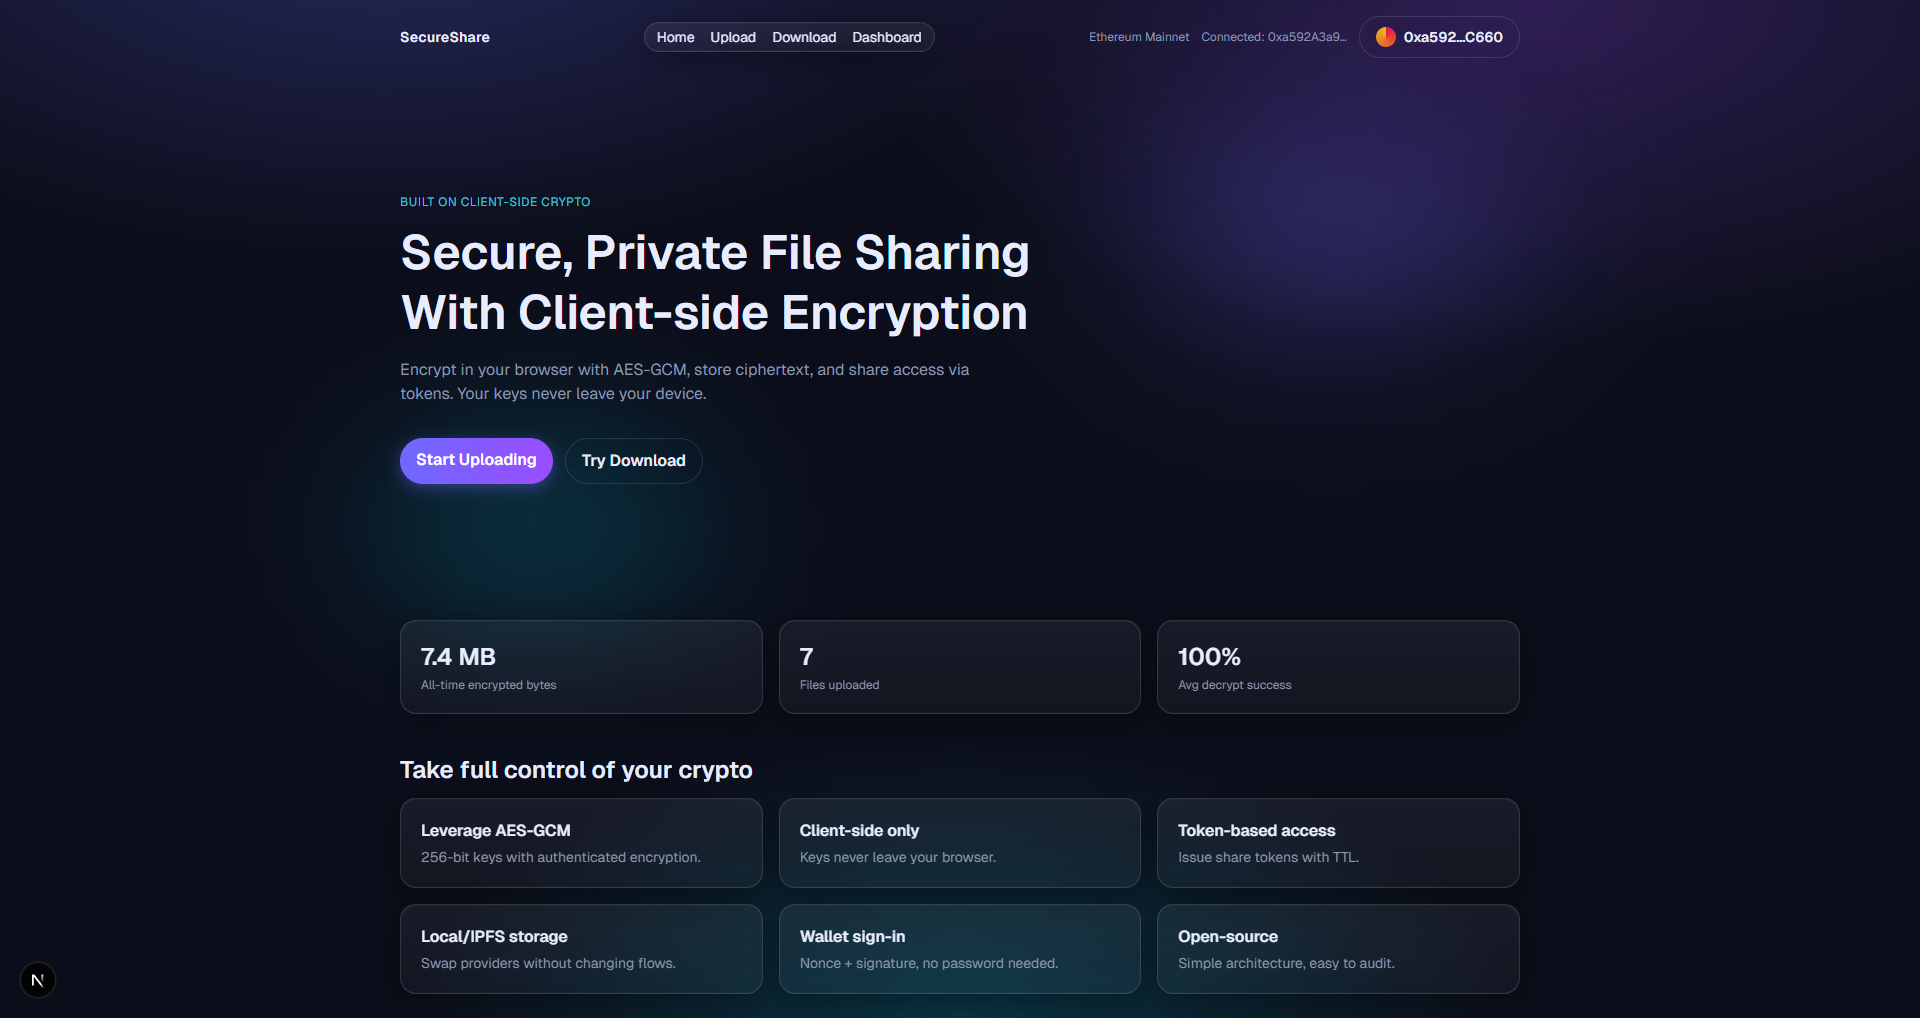
\includegraphics[width=\linewidth]{ui-home.png}
    \caption{Home Page with Hero Section}
  \end{subfigure}\hfill
  \begin{subfigure}{0.48\textwidth}
    \centering
    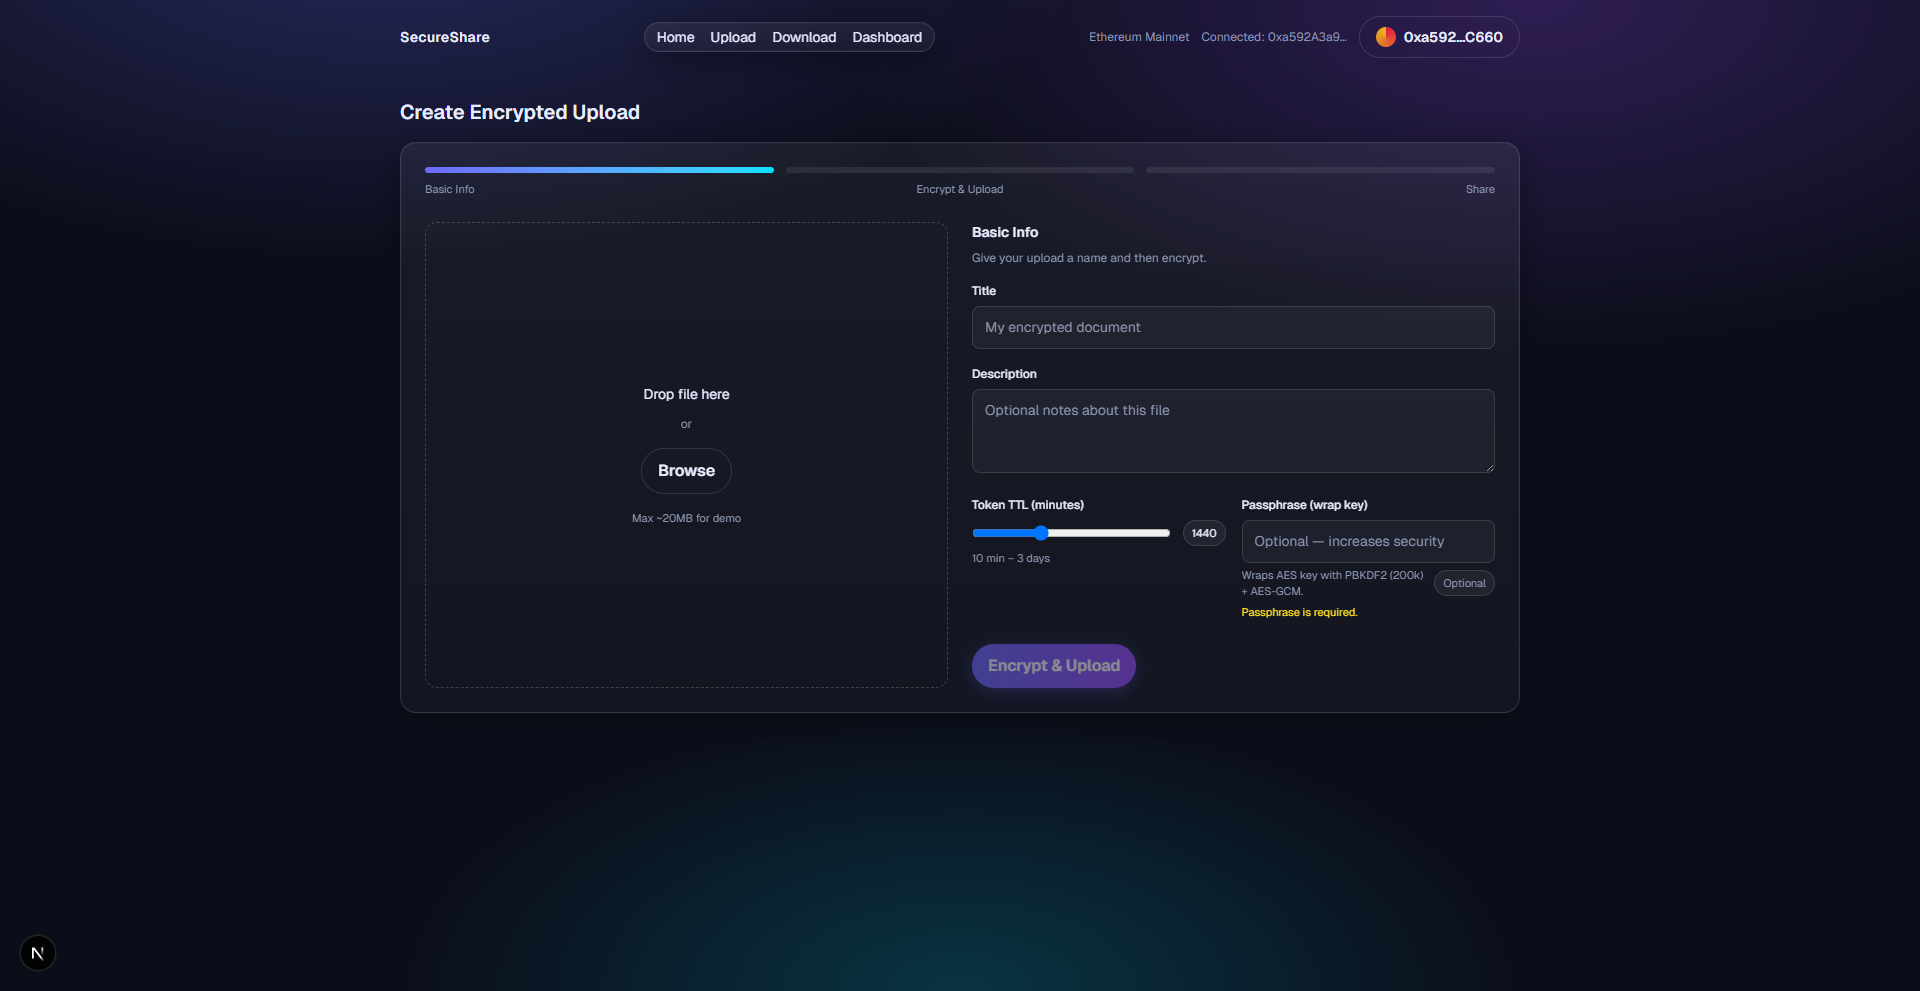
\includegraphics[width=\linewidth]{ui-upload.png}
    \caption{Upload Page with Encryption Wizard}
  \end{subfigure}
  \caption{Application Interface - Part 1}
\end{figure}

\begin{figure}[H]
  \centering
  \begin{subfigure}{0.48\textwidth}
    \centering
    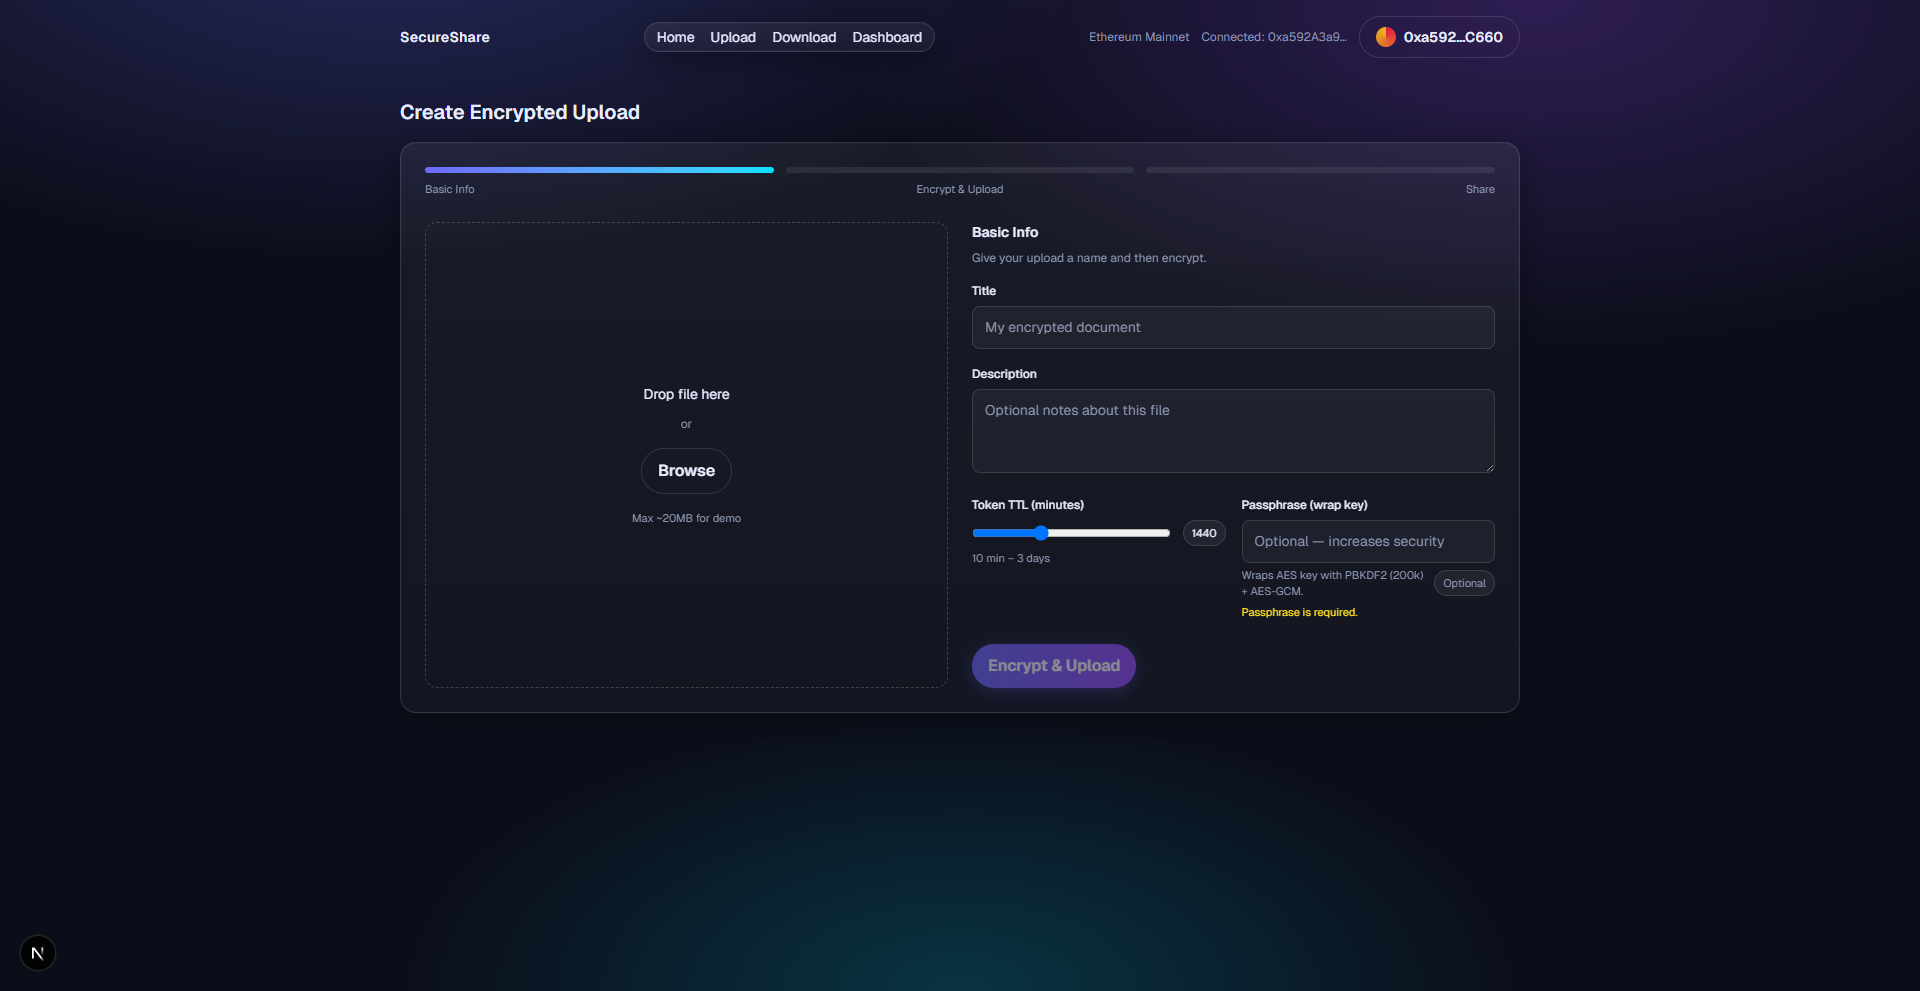
\includegraphics[width=\linewidth]{ui-download.png}
    \caption{Download \& Decrypt Page}
  \end{subfigure}\hfill
  \begin{subfigure}{0.48\textwidth}
    \centering
    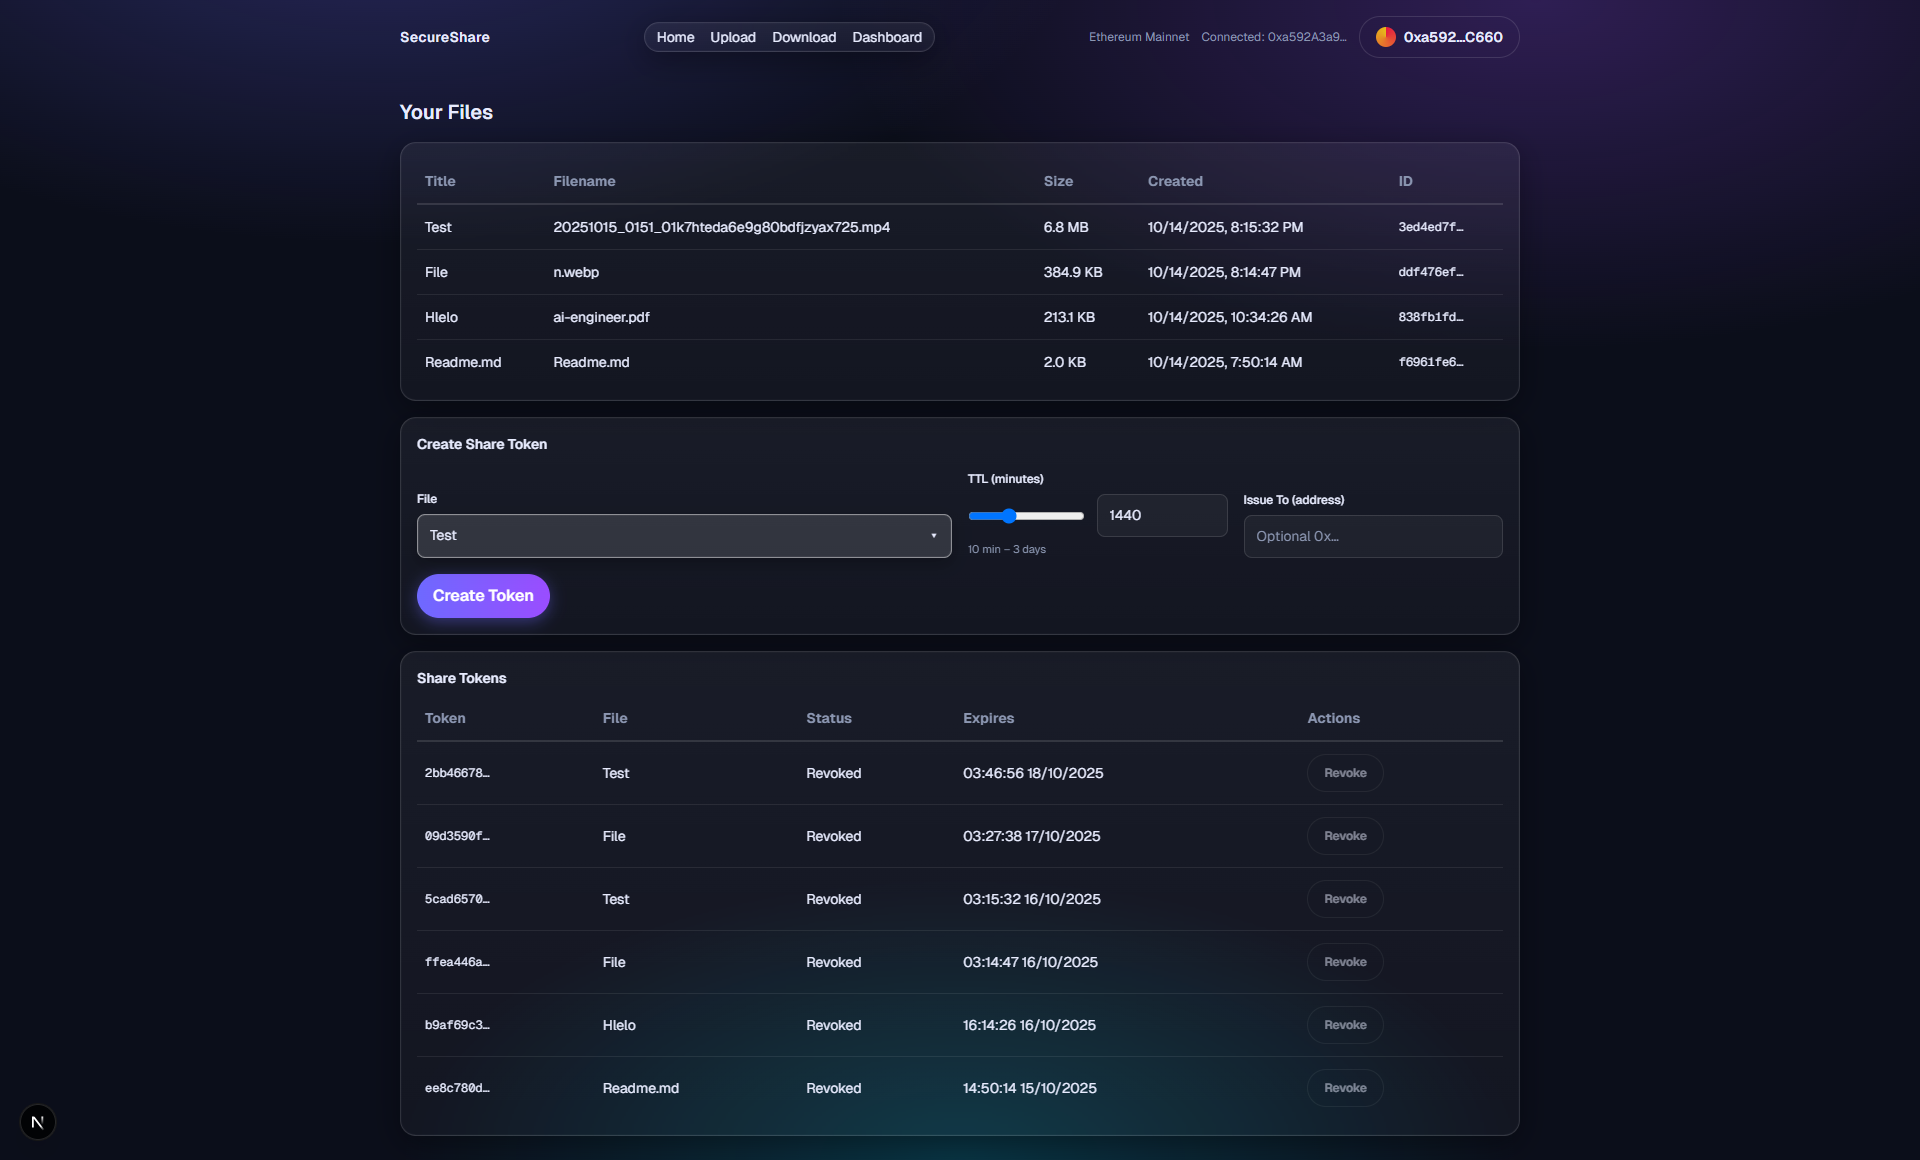
\includegraphics[width=\linewidth]{ui-dashboard.png}
    \caption{Dashboard with File Management}
  \end{subfigure}
  \caption{Application Interface - Part 2}
\end{figure}

\section{Installation \& Setup}
\subsection*{Prerequisites}
\begin{itemize}
  \item Node.js v18 or higher
  \item npm v9 or higher
  \item MetaMask browser extension (for wallet integration)
\end{itemize}

\subsection*{Installation Steps}
\begin{enumerate}
  \item Clone or extract the project repository
  \item Navigate to the project root directory
  \item Run \texttt{npm install} to install dependencies
  \item Create \texttt{.env.local} file with required environment variables
  \item Run \texttt{npm run dev} to start the development server
  \item Open \texttt{http://localhost:3000} in your browser
\end{enumerate}

\section{User Guide}
\subsection*{1. Connecting Your Wallet}
To use the application, connect your Ethereum wallet (MetaMask):
\begin{enumerate}
  \item Click the \textbf{``Connect Wallet''} button in the top-right corner
  \item MetaMask will open; select your account and approve the connection
  \item Sign the authentication message (nonce) to verify ownership
  \item Your wallet address will appear in the header
\end{enumerate}

\subsection*{2. Uploading and Encrypting a File}
To upload a file with encryption:
\begin{enumerate}
  \item Navigate to the \textbf{Upload} page
  \item Drag and drop a file or click \textbf{Browse} to select one
  \item Enter a \textbf{Title} and optional \textbf{Description}
  \item (Optional) Enter a \textbf{Passphrase} to wrap the AES key (recommended for production)
  \item Adjust \textbf{Token TTL} (time-to-live) from 10 minutes to 3 days
  \item Click \textbf{Encrypt \& Upload}
  \item The file is encrypted client-side using AES-256-GCM; only ciphertext is sent to the server
  \item A share token is generated and displayed
\end{enumerate}

\subsection*{3. Sharing the File}
After uploading:
\begin{enumerate}
  \item Copy the \textbf{Share Token} or \textbf{Download Link}
  \item Send the token/link to the recipient via any communication channel
  \item The recipient can use the token to download and decrypt the file
  \item Tokens can be revoked at any time from the Dashboard
\end{enumerate}

\subsection*{4. Downloading and Decrypting a File}
To decrypt and download a shared file:
\begin{enumerate}
  \item Navigate to the \textbf{Download} page (or use the share link directly)
  \item Paste the \textbf{Token} into the input field
  \item Click \textbf{Validate} to check token validity and retrieve file metadata
  \item If the file was wrapped with a passphrase, enter it
  \item Click \textbf{Download \& Decrypt} to download the decrypted file
  \item The decryption happens entirely in your browser; the server never sees the decrypted content
\end{enumerate}

\subsection*{5. Managing Files and Tokens}
On the \textbf{Dashboard}:
\begin{itemize}
  \item View all files you have uploaded (owner only)
  \item See file details: name, size, upload date
  \item Issue new tokens for any of your files
  \item Revoke existing tokens to immediately disable access
  \item Manage token TTL and optionally restrict tokens to specific addresses
\end{itemize}


\chapter{Kiểm thử và đánh giá}

\section{Tiêu chí đánh giá}
\begin{itemize}
  \item \textbf{Đúng chức năng}: mã hoá/giải mã chính xác; token hoạt động, TTL/thu hồi hợp lệ.
  \item \textbf{Bảo mật}: không rò rỉ khoá; kiểm tra CSRF; từ chối token sai/hết hạn.
  \item \textbf{Hiệu năng}: thời gian mã hoá/giải mã và tải tệp trong ngưỡng chấp nhận được.
\end{itemize}

\section{Phân tích rủi ro và giảm thiểu}
\begin{itemize}
  \item \textbf{IV trùng lặp}: sinh ngẫu nhiên 96‑bit; tuyệt đối không tái sử dụng IV cùng khoá.
  \item \textbf{Passphrase yếu}: gợi ý độ mạnh, khuyến nghị tối thiểu 12 ký tự, PBKDF2 200k vòng.
  \item \textbf{Rò rỉ khoá (chế độ demo)}: tắt \texttt{ALLOW\_RAW\_KEYS} trong sản xuất; dùng wrappedKey bắt buộc.
  \item \textbf{Tấn công CSRF/XSRF}: header \texttt{x-csrf} + cookie cùng giá trị; kiểm tra phía server.
\end{itemize}


\chapter{Kết luận và hướng phát triển}

\section{Kết luận}
Đề tài đã chứng minh tính khả thi của mô hình chia sẻ tệp bảo mật với mã hoá phía client (client-side encryption). Bằng cách lưu trữ ciphertext trên máy chủ và chỉ giữ metadata, hệ thống đạt được mục tiêu \textbf{zero-knowledge}: máy chủ không bao giờ biết được nội dung hoặc khóa giải mã của tệp.

\subsection*{Những thành tựu chính}
\begin{itemize}
  \item \textbf{Mã hoá an toàn}: Triển khai thành công AES-256-GCM với Web Crypto API; tất cả khóa được tạo và quản lý phía client.
  \item \textbf{Xác thực không mật khẩu}: Sử dụng chữ ký Ethereum (MetaMask) để xác thực, loại bỏ nhu cầu lưu trữ mật khẩu phía server.
  \item \textbf{Kiểm soát quyền truy cập}: Token-based access control với TTL (time-to-live) và khả năng thu hồi ngay lập tức.
  \item \textbf{Bảo vệ CSRF}: Triển khai double-submit cookie pattern và SameSite cookie để bảo vệ các endpoint thay đổi trạng thái.
  \item \textbf{Giao diện thân thiện}: Ứng dụng web hiện đại với flow trực quan cho upload, tạo token, và download.
\end{itemize}

\subsection*{Những thách thức gặp phải}
\begin{itemize}
  \item \textbf{Tương thích trình duyệt}: Web Crypto API có hỗ trợ tốt nhưng cần kiểm tra polyfill cho các trình duyệt cũ hơn.
  \item \textbf{Hiệu năng}: Mã hoá/giải mã các tệp lớn phía client có thể mất nhiều thời gian; cần tối ưu hóa UI để hiển thị tiến độ.
  \item \textbf{Trải nghiệm người dùng}: Cân bằng giữa bảo mật (yêu cầu passphrase) và dễ sử dụng (tùy chọn passphrase).
  \item \textbf{Lưu trữ}: Triển khai hiện tại sử dụng lưu trữ cục bộ; scaling lên IPFS/Filecoin đòi hỏi nghiên cứu thêm.
\end{itemize}

\subsection*{Lesson Learned}
\begin{itemize}
  \item Lựa chọn thuật toán đúng (AES-GCM) quan trọng hơn tối ưu hóa tùy ý; tiêu chuẩn công nghiệp cung cấp độ tin cậy tốt.
  \item Quản lý khoá là phần khó nhất: cần cân nhắc kỹ cách lưu trữ, sao lưu, và khôi phục.
  \item Bảo mật phía server (CSRF, input validation, rate limiting) cũng quan trọng như bảo mật phía client.
  \item Testing bảo mật cần phải toàn diện: unit tests, integration tests, và manual penetration testing.
\end{itemize}

\section{Hướng phát triển}
Để nâng cấp dự án lên mức độ sản xuất và mở rộng các tính năng, các công việc sau được đề xuất:

\subsection*{Ngắn hạn (1-2 tháng)}
\begin{enumerate}
  \item \textbf{Bắt buộc passphrase}: Loại bỏ chế độ demo `ALLOW_RAW_KEYS`; yêu cầu PBKDF2-wrapped key bắt buộc.
  \item \textbf{Performance optimization}: Implement Web Worker để mã hoá/giải mã không chặn UI.
  \item \textbf{Mobile responsiveness}: Tối ưu hoá giao diện cho các thiết bị di động.
  \item \textbf{Comprehensive testing}: Thêm unit tests, integration tests, và E2E tests với Playwright.
\end{enumerate}

\subsection*{Trung hạn (3-6 tháng)}
\begin{enumerate}
  \item \textbf{IPFS integration}: Thay thế lưu trữ cục bộ bằng IPFS hoặc Filecoin để phân tán hóa lưu trữ.
  \item \textbf{Attribute-Based Access Control (ABAC)}: Hỗ trợ chia sẻ dựa trên thuộc tính (ví dụ: địa chỉ ví, role).
  \item \textbf{Audit logging}: Ghi lại tất cả các hoạt động (upload, token issuance, revocation) cho mục đích kiểm toán.
  \item \textbf{Multi-signature support}: Cho phép yêu cầu từ nhiều ví để phê duyệt chia sẻ.
\end{enumerate}

\subsection*{Dài hạn (6+ tháng)}
\begin{enumerate}
  \item \textbf{Smart contract integration}: Triển khai hợp đồng thông minh on-chain (Ethereum, Polygon, etc.) để quản lý tokens và quyền truy cập.
  \item \textbf{Mobile app}: Phát triển ứng dụng di động native cho iOS/Android với xác thực sinh trắc học.
  \item \textbf{Decentralized naming}: Hỗ trợ ENS (Ethereum Name Service) để thay thế địa chỉ ví dài.
  \item \textbf{Cross-chain compatibility}: Hỗ trợ xác thực từ các blockchain khác nhau.
\end{enumerate}

\subsection*{Chất lượng & Bảo mật}
\begin{enumerate}
  \item \textbf{Security audit}: Nhờ audit bên thứ ba cho code và cryptography.
  \item \textbf{Bug bounty program}: Mở chương trình bounty để khuyến khích researcher tìm lỗ hổng.
  \item \textbf{Documentation}: Cải thiện tài liệu API, architecture docs, và security guidelines.
  \item \textbf{Compliance}: Đảm bảo tuân thủ GDPR, CCPA, và các quy định bảo vệ dữ liệu khác.
\end{enumerate}


% Simple manual bibliography
\begin{thebibliography}{9}
  \bibitem{NISTAES} NIST FIPS 197. Advanced Encryption Standard (AES), 2001.
  \bibitem{NISTGCM} NIST SP 800‑38D. Galois/Counter Mode (GCM) and GMAC, 2007.
  \bibitem{RFC2898} IETF RFC 2898. PKCS \#5: PBKDF2, 2000.
  \bibitem{RFC7519} IETF RFC 7519. JSON Web Token (JWT), 2015.
  \bibitem{WebCrypto} W3C. Web Cryptography API, Recommendation.
\end{thebibliography}



\end{document}

